%versi 2 (8-10-2016)
\chapter{Landasan Teori}
\label{chap:teori}

\lstdefinelanguage{JavaScript}{
  keywords={typeof, new, true, false, catch, function, return, null, catch, switch, var, if, in, while, do, else, case, break},
  keywordstyle=\color{blue}\bfseries,
  ndkeywords={class, export, boolean, throw, implements, import, this},
  ndkeywordstyle=\color{gray}\bfseries,
  identifierstyle=\color{black},
  sensitive=false,
  comment=[l]{//},
  morecomment=[s]{/*}{*/},
  commentstyle=\itshape\color{green},
  stringstyle=\color{red},
  morestring=[b]',
  morestring=[b]"
}

\lstset{
   language=JavaScript,
   backgroundcolor=\color{white},
   extendedchars=true,
   basicstyle=\fontfamily{fvm}\selectfont\small, 
   showstringspaces=false,
   showspaces=false,
   numbers=left,
   numberstyle=\footnotesize,
   numbersep=5pt,
   tabsize=4,
   breaklines=true,
   showtabs=false,
   captionpos=b,
   frame=leftline,
   stepnumber=1,
   literate={-}{-}1{-\,-}{--}1
}

\section{\textit{Snake}}
\label{sec:snake}
\textit{Snake} merupakan permainan mengendalikan ular untuk mendapatkan makanan yang terdapat pada labirin. Dalam permainan ini, pemain mengendalikan ular untuk mendapatkan makanan sebanyak-banyaknya. Setiap ular memakan makanan, maka skor akan bertambah 1 poin dan tubuh ular akan bertambah panjang. Biasanya makanan hanya ada 1 saja pada sebuah labirin. Ketika makanan itu sudah termakan oleh ular, makanan tersebut akan ditempatkan secara acak. Ular dapat bergerak ke atas, bawah, kiri, dan kanan. Namun pada permainan \textit{Snake} yang akan dibuat sekarang, ular dapat bergerak ke segala arah seperti ilustrasi pada Gambar~\ref{fig:ularSegalaArah}. Permainan akan berakhir jika ular menabrak dinding yang terdapat pada labirin atau ular tersebut menabrak tubuhnya sendiri. \\

\begin{figure}[H]
	\centering  
	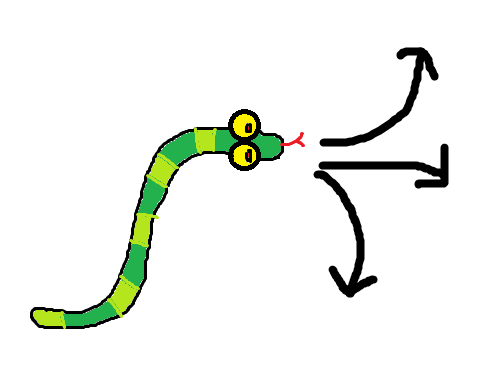
\includegraphics[scale=0.4]{ular-segala-arah}  
	\caption[Pergerakan ular ke segala arah]{Pergerakan ular ke segala arah} 
	\label{fig:ularSegalaArah} 
\end{figure} 

Permainan \textit{Snake} ini dapat dimainkan secara \textit{singleplayer} atau \textit{multiplayer}. \textit{Singleplayer game} adalah permainan yang dapat dimainkan oleh 1 pemain. \textit{Multiplayer game} adalah permainan yang dapat dimainkan oleh beberapa pemain. Pada umumnya, permainan \textit{Snake} dimainkan secara \textit{singleplayer}. Contoh \textit{singleplayer game Snake} adalah \textit{Snake} pada telepon genggam \textit{Nokia} yang dapat dilihat pada Gambar~\ref{fig:nokiaSnake}\footnote{https://en.wikipedia.org/wiki/Snake\_(video\_ game\_ genre)} dan contoh \textit{multiplayer game Snake} adalah \textit{Slither.io} yang dapat dilihat Gambar~\ref{fig:slither}\footnote{https://play.google.com/store/apps/details?id=air.com.hypah.io.slither}. \textit{Snake} dapat dimainkan menggunakan \textit{smartphone} dan \textit{web browser}.  

\begin{figure}[H]
	\centering  
	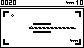
\includegraphics[scale=2]{nokiaSnake}  
	\caption[Permainan Snake pada telepon genggam \textit{Nokia}]{Permainan Snake pada telepon genggam \textit{Nokia}} 
	\label{fig:nokiaSnake} 
\end{figure} 

\begin{figure}[H]
	\centering  
	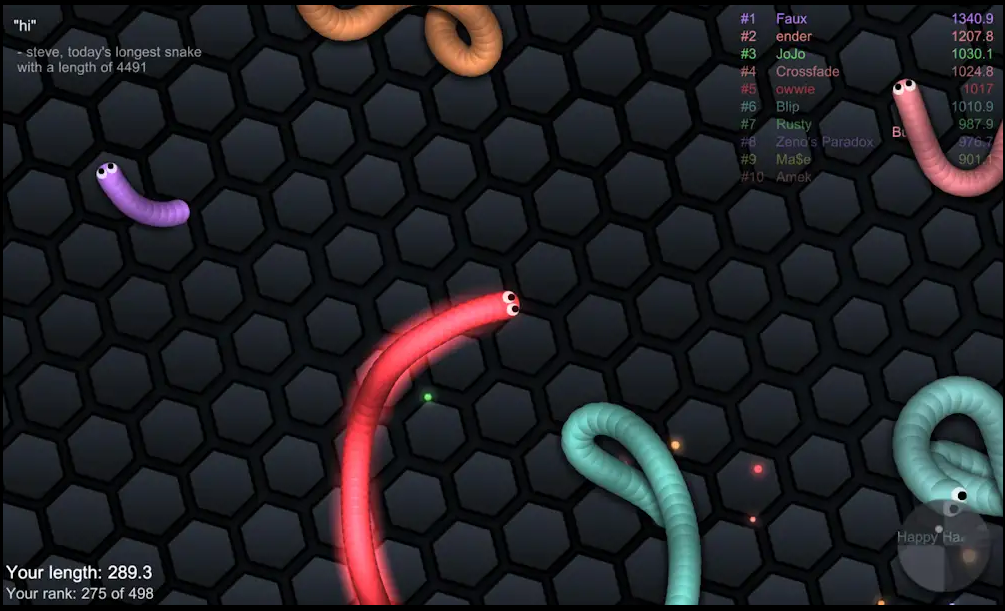
\includegraphics[scale=0.3]{slither}  
	\caption[Permainan \textit{Slither.io} pada \textit{Android}]{Permainan \textit{Slither.io} pada \textit{Android}} 
	\label{fig:slither} 
\end{figure} 

\section{HTML5 \textit{Canvas}}
\label{sec:HTML5Canvas}
HTML5 Canvas adalah sebuah daerah \textit{bitmap} yang dapat dimanipulasi oleh \textit{Javascript}. Pada daerah \textit{bitmap} tersebut, \textit{pixel-pixel} akan di\textit{render} oleh canvas. Setiap \textit{frame}, HTML5 Canvas akan menggambar pada area \textit{bitmap} tersebut menggunakan \textit{Canvas} API(\textit{Application Programming Interface}) yang dipanggil pada \textit{Javascript}. API dari HTML5 Canvas yang umum adalah 2D \textit{Context}. Dengan adanya 2D \textit{Context}, \textit{programmer} dapat membuat bentuk 2D, menampilkan gambar, \textit{render} tulisan, memberi warna, membuat garis dan kurva, dan manipulasi \textit{pixel}. HTML5 Canvas tidak hanya digunakan untuk menggambar dan menampilkan gambar serta tulisan. HTML5 Canvas dapat digunakan untuk membuat animasi, aplikasi pada \textit{web} dan permainan. 

Untuk menambahkan \textit{canvas} pada halaman HTML, diperlukan \textit{tag} <canvas>. Di bawah ini adalah potongan kode untuk menambahkan \textit{canvas} pada halaman HTML. \textbf{YANG CONTEXT HARUS DIMASUKIN DI SINI ATAU DI JAVASCRIPT?}

\begin{lstlisting}[language=HTML]
	<canvas id='canvas' width='500' height='300'>
		Your browser does not support HTML5 Canvas.
	</canvas>
	
\end{lstlisting}

Berikut adalah penjelsan atribut yang ada pada \textit{canvas} berdasarkan potongan kode di atas : \textbf{DIISI!}


\section{\textit{\textit{Javascript}}}
\label{sec:Javascript}
\textit{Javascript} adalah bahasa pemrograman yang ringan, \textit{interpreted} dan berorientasi objek yang digunakan pada halaman \textit{web}. \textit{Javascript} dapat membuat objek dengan menambahkan \textit{method} dan atributnya sama seperti bahasa pemrograman C++ dan \textit{Java}. Setelah objek diinisialisasi, maka objek tersebut dapat dijadikan \textit{blueprint} untuk membuat objek lain yang mirip\footnote{https://developer.mozilla.org/en-US/docs/Web/JavaScript/About\_ JavaScript}. \textit{Javascript} dapat digunakan untuk mengimplementasi hal yang kompleks pada halaman web. Contohnya adalah menamplikan peta yang interaktif dan membuat animasi 2D/3D. Selain \textit{Javascript}, HTML(\textit{HyperText Markup Language}) dan CSS(\textit{Cascading Style Sheet}) merupakan bagian/komponen penting dalam pembuatan halaman \textit{web}\footnote{https://developer.mozilla.org/en-US/docs/Learn/JavaScript/First\_ steps/What\_ is\_ JavaScript}.\\

\subsection{Fitur Utama pada \textit{Javascript}}
\textit{Javascript} memiliki fitur utama yang umum dikenal pada bahasa pemrograman lainya. Fitur-fitur utama tersebut adalah variabel, komentar, \textit{function}, \textit{conditional} dan operator. 

\subsubsection{Variabel}


\subsection{Menggambar pada \textit{Canvas}}
Sesudah menuliskan \textit{tag} <canvas> pada HTML, canvas tidak bisa langsung digambar. Karena itu perlu ditambahkan \textit{drawing context} pada \textit{Javascript}. Di bawah ini adalah potongan kode untuk menambahkan \textit{drawing context}.

\begin{lstlisting}
	var myCanvas = document.getElementById('canvas');
	var context = myCanvas.getContext('2d');
\end{lstlisting}

Berdasarkan potongan kode di atas, variabel myCanvas menyimpan objek dengan id = 'canvas'. Id ini mengacu ke objek \textit{canvas} yang pada potongan kode sebelumnya. Variabel myCanvas sekarang sudah menyimpan objek \textit{canvas}. Kemudian variabel context menyimpan \textit{drawing context} 2D. Sesudah itu, \textit{canvas} tersebut dapat digambar dengan bentuk 2D, garis, kurva, membuat tulisan, dan menambahkan gambar. Selain untuk menggambar, bentuk-bentuk tersebut dapat diberi warna sesuai dengan keinginan.\\

Untuk menggambar bentuk 2D atau garis, diperlukan koordinat x dan y. Koordinat tersebut akan menempatkan gambar tersebut pada \textit{canvas}. Posisi awal/\textit{origin} pada \textit{canvas} adalah (0,0) yang terletak di ujung kiri atas \textit{canvas}. Gambar~\ref{fig:grid} adalah penempatan kotak biru pada \textit{canvas} terhadap \textit{origin}.

\begin{figure}[H]
	\centering  
	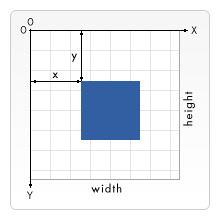
\includegraphics[scale=0.5]{grid}
	\caption[Posisi kotak biru pada \textit{canvas} terhadap \textit{origin}]{Posisi kotak biru pada \textit{canvas} terhadap \textit{origin}}
	\label{fig:grid} 
\end{figure} 

Pada Gambar~\ref{fig:grid}, titik ujung kiri kotak biru tersebut berjarak x \textit{pixel} dari kiri dan berjarak y \textit{pixel} dari atas. 

\subsubsection{Menggambar Bentuk Persegi Panjang}
Ada 3 cara untuk menggambar persegi panjang:

\begin{itemize}
	\item \textit{fillRect(x,y,width,height)} : menggambar persegi panjang serta mengisi bagian tengah persegi panjang.
	\item \textit{strokeRect(x,y,width,height)} : menggambar \textit{outline} yang berbentuk persegi panjang.
	\item \textit{clearRect(x,y,width,height)} : menghapus daerah yang ditentukan pada \textit{canvas}. Daerah yang dihapus berbentuk persegi panjang.
\end{itemize}

Fungsi tersebut memiliki parameter yang sama. Parameter x dan y untuk menentukan posisi pada canvas dari titik ujung kiri atas persegi panjang. \textit{Width} adalah lebar dari persegi panjang dan \textit{height} adalah tinggi dari persegi panjang.

\subsubsection{Menggambar \textit{Path}}
\textit{Path} adalah sekumpulan titik yang dihubungkan oleh segmen garis. \textit{Path} dapat membentuk kurva dan membuat bentuk 2D lainnya seperti segitiga, trapesium, belah ketupat dan lain-lain. Langkah-langkah untuk membuat bentuk menggunakan path adalah sebegai berikut : 

\begin{enumerate}
	\item Buat \textit{path}.
	\item Tuliskan perintah untuk menggambar pada \textit{path} tersebut.
	\item Sesudah \textit{path} tersebut sudah dibuat, \textit{path} tersebut dapat di\textit{render} menggunakan \textit{stroke} atau \textit{fill}.
\end{enumerate}



\subsection{Membuat Objek pada \textit{Javascript}}
\textit{Javascript} mendukung OOP(\textit{Object Oriented Programming}) sehingga \textit{programmer} lebih mudah mengerti cara kerja program tersebut. \textit{Object Oriented Programming} merupakan paradigma pemrograman berdasarkan konsep objek\footnote{https://id.wikipedia.org/wiki/Pemrograman\_ berorientasi\_ objek}. Objek tersebut dapat berupa benda-benda yang ada pada kehidupan sehari-hari. Setiap objek memiliki atribut dan \textit{method}. Atribut adalah data dan karakteristik yang terdapat pada objek. \textit{Method} adalah hal yang dapat dilakukan oleh objek tersebut. Contohnya, objek mobil memiliki atribut warna mobil, merk mobil, dan berat mobil. \textit{Method} objek mobil adalah dapat berbelok, dapat berhenti dan dapat maju. \\

Pada \textit{Javascript} untuk membuat objek, digunakan perintah \textit{function}. Pada Gambar~\ref{fig:objectFunctionCode} adalah potongan kode untuk membuat objek pada \textit{Javascript} dengan atribut dan \textit{method}.

\begin{figure}[H]
	\centering  
	\includegraphics[scale=1]{objectFunctionCode}
	\caption[Membuat objek pada \textit{Javascript}]{Membuat objek pada \textit{Javascript}}
	\label{fig:objectFunctionCode} 
\end{figure} 

Berdasarkan potongan kode pada Gambar~\ref{fig:objectFunctionCode}, objek mobil tersebut memiliki atribut yaitu merk mobil, warna mobil dan berat mobil. \textit{Method} dari objek mobil adalah mobil dapat berbelok ke kanan dan ke kiri.

\subsection{\textit{Events}}
\textit{Event} adalah sebuah cara untuk membuat halaman web menjadi lebih interaktif. Javascript akan menjalankan suatu hal apabila \textit{event} tersebut terdeteksi\footnote{https://www.w3schools.com/js/js\_ events.asp}. Misalnya apabila sebuah tombol ditekan pada \textit{web browser}, maka akan muncul tanggal hari ini.  Pada skripsi ini, event yang digunakan adalah event milik \textit{jQuery} dan \textit{event keyboard} akan digunakan. Setiap tombol pada \textit{keyboard} memiliki kode unik/\textit{key code} tersendiri. \textit{Event-event} yang digunakan adalah sebagai berikut:

\begin{itemize}
	\item \textit{keydown} : fungsi akan dieksekusi apabila pengguna menekan sebuah tombol.
	\item \textit{keyup} : fungsi akan dieksekusi apabila pengguna sedang tidak menekan sebuah tombol.
\end{itemize}

Kode-kode pada \textit{keyboard} yang digunakan adalah tombol atas, bawah, kanan dan kiri. Pada Gambar~\ref{fig:eventKeyDown} adalah potongan kode untuk membuat \textit{event keydown}.

\begin{figure}[H]
	\centering  
	\includegraphics[scale=1]{eventKeydown}
	\caption[\textit{Event keydown} pada tombol atas, bawah, kiri, dan kanan]{\textit{Event keydown} pada tombol atas, bawah, kiri, dan kanan}
	\label{fig:eventKeyDown} 
\end{figure} 

\subsection{Membuat Animasi}
\textit{Javascript} dan \textit{jQuery} dapat digunakan untuk membuat animasi. Animasi adalah proses pergantian gambar yang hampir berbeda satu dengan yang lainya secara cepat sehingga gambar tersebut seolah-olah bergerak\footnote{https://en.wikipedia.org/wiki/Animation}. Langkah-langkah untuk membuat animasi menggunakan canvas adalah :

\begin{itemize}
	\item \textit{Draw} : gambar objek tersebut
	\item \textit{Update} : \textit{update} posisi dari objek tersebut.
	\item \textit{Clear} : hapus semua objek yang ada pada canvas.
	\item \textit{Repeat} : lakukan 3 hal diatas secara berulang.
\end{itemize}

Untuk membuat animasi, membutuhkan perintah \textit{setTimeout}. \textit{setTimeout} dapat membatasi \textit{framerate} sehingga animasi tidak bergerak terlalu cepat. Sintaks untuk \textit{setTimeout} adalah setTimeout(x,y), di mana x adalah sebuah fungsi yang ingin dibuat animasi dan y adalah \textit{framerate} dari animasi tersebut. Gambar~\ref{fig:animate} menunjukan cara untuk membuat animasi. Fungsi \textit{animate()} di baris paling akhir harus dipanggil lagi supaya animasi dapat berjalan terus-menerus.

\begin{figure}[H]
	\centering  
	\includegraphics[scale=1]{animate}
	\caption[Membuat kotak berpindah posisi]{Membuat kotak berpindah posisi}
	\label{fig:animate} 
\end{figure} 

\section{\textit{jQuery}}
\textit{jQuery} adalah pustaka yang dimiliki oleh \textit{Javascript}. Semua perintah-perintah pada \textit{Javascript} dapat digunakan oleh \textit{jQuery}. Penulisan \textit{jQuery} lebih singkat dibandingkan \textit{Javascript}.

Di bawah ini adalah potongan kode pada \textit{jQuery}. Untuk mendapatkan objek pada \textit{jQuery} selalu diawali dengan simbol '\$'. Kemudian diikuti dengan objeknya lalu \textit{method}nya. 

\begin{lstlisting}
	$( "h1" ).remove();
	
\end{lstlisting}

\textit{jQuery} dapat mendeteksi apakah halaman \textit{web} sudah siap atau belum. Potongan kode di bawah ini adalah untuk mendeteksi halaman \textit{web}.

\begin{lstlisting}
	$( document ).ready(function() {
    	// kode dituliskan di sini
	});
	
\end{lstlisting}

Kode yang dituliskan di dalam \$( document ).ready(function() akan dijalan setelah DOM(\textit{Document Object Model}) pada halaman web tersebut sudah siap untuk dieksekusi oleh \textit{Javascript}. 

\section{\textit{Git}}
\label{sec:Git}
\textit{Github} adalah layanan \textit{web hosting} bersama untuk proyek pengembangan perangkat lunak yang menggunakan sistem \textit{version control} yaitu \textit{Git}\footnote{https://en.wikipedia.org/wiki/GitHub}. \textit{Git} dapat mengetahui perubahan pada file di komputer. \textit{Github} biasanya digunakan oleh para \textit{programmer} untuk menambahkan/merevisi \textit{source code} dan sebagai media untuk berkolaborasi dalam proyek pembangunan perangkat lunak. \textit{Source code} tersebut disimpan dikelompokan pada file dan file tersebut disimpan di\textit{repository}. Dalam 1 \textit{repository}, \textit{owner}(pengguna yang membuat \textit{repository}) dapat mengundang pengguna lain untuk berkolaborasi. Ketika ada perubahan pada \textit{repository}, maka \textit{collaborator}(pengguna yang diberi hak untuk mengubah \textit{repository}) dapat mengetahui \textit{source code} atau file yang direvisi oleh \textit{collaborator} lain.\\

\textit{Github} memiliki banyak fitur untuk memudahkan kerja \textit{programmer}. Fitur \textit{Github} yang mendukung penelitian ini adalah \textit{pull request}. \textit{Pull request} memberitahu \textit{collaborator} lain tentang perubahan pada \textit{repository}. Dengan adanya \textit{pull request}, pengguna dan \textit{collaborator} lain dapat berdiskusi tentang perubahan tersebut. Perubahan tersebut harus di \textit{merge} oleh \textit{collaborator} dari \textit{repository}. Apabila sudah di \textit{merge} oleh \textit{collaborator}, perubahan tersebut akan disimpan di \textit{repository}\footnote{https://help.github.com/articles/about-pull-requests}.